\subsubsection{Regressione}

Procediamo ora con l'analisi del grafico del dislivello $d$ in funzione della temperatura $\theta$. In base ai dati da noi raccolti abbiamo ottenuto il seguente risultato, illustrato in figura (\ref{fig:dislivello_temperatura})

\begin{SCfigure}
    \centering
    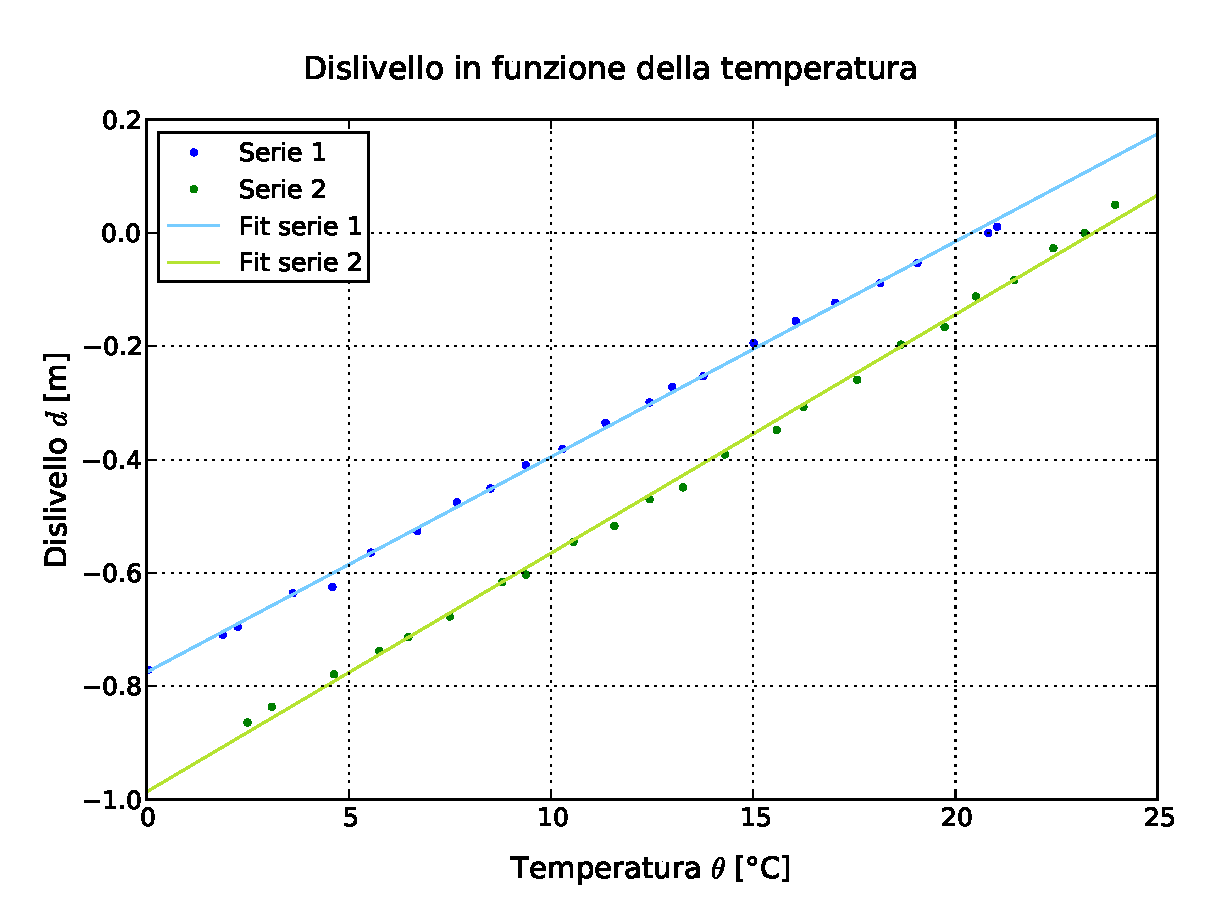
\includegraphics[width=110mm]{immagini/dislivello_temperatura.pdf}
    \caption{Il seguente grafico rappresenta}
    \label{fig:dislivello_temperatura}
\end{SCfigure}
%
Quindi in base a questi dati noi vogliamo verificare che la legge di prporzionalità diretta che lega la temperatura $\theta$ con il dislivello $d$ della colonnina di acqua sia corretta. Pertanto la legge si presenta come segue:

\begin{equation}
	h \,=\, A + B\,\theta
	\label{h_theta}
\end{equation}
%
